\documentclass[a4paper]{article}
\usepackage[utf8]{inputenc} % para poder usar tildes en archivos UTF-8
\usepackage[spanish]{babel} % para que comandos como \today den el resultado en castellano
\usepackage{a4wide} % márgenes un poco más anchos que lo usual
\usepackage[showRevisiones]{caratula}
\usepackage{xcolor}
\usepackage{listings}
\lstset{basicstyle=\ttfamily,
  showstringspaces=false,
  commentstyle=\color{red},
  keywordstyle=\color{blue}
}

\begin{document}

\materia{Organización de Computadoras 66.20}
\tipoapunte{Trabajo Práctico #1}

\fecha{\today}

\autor{Flórez Del Carpio, Christian}{91011}{chris.florez.d.c@gmail.com}
\autor{Montenegro, Josefina}{94289}{mariajosefina.mont@gmail.com}
\autor{Quino López, Julián}{94224}{julianquino2@gmail.com}

\revision{10/10/2017}{-}{Entrega primera versión del TP}
\maketitle

\begin{abstract}
El siguiente trabajo práctico tiene como objetivo familiarizarse con el conjunto de instrucciones MIPS y el concepto de ABI, para lograr dicho propósito se debe implementar la lógica de detección de palíndromos en assembly, entendiendo como palabras a aquellas compuestas por letras [A-Z], números [0-9], guiones bajos y medios, es decir, cualquier combinación posible de los anteriormente mencionados, tal como estaba enunciado en el TP0.
\end{abstract}


\section{Introducción}
Pueden haber tres escenarios posibles, el caso en el cual el usuario ingresa archivo de entrada y salida, el caso en el que se ingresa un archivo de entrada solamente y por último el caso donde se recibe el archivo de salida. En caso de no proporcionar un archivo de texto como entrada, se requerirá ingresar el stream por entrada standard. Si no se especifica un archivo de salida, se mostrarán los resultados por salida standard. Esto es igual a lo explicando en el TP0.


\section{Desarrollo}

Se desarrolló un programa C, desde el cual se invoca a la función palindrome escrita en assembly. Esta función recibe como parámetros los archivos de entrada/salida (si no se hubiesen proporcionado tales archivos se toman los streams de entrada/salida standard) y las cantidades ibytes y obytes, las cuales describen la unidad de transferencia para escribir en el buffer de entrada/salida, respectivamente. Cuando no son proporcionados estos valores, se toma por defecto el valor 1.

\subsection{Comandos para compilar y ejecutar el programa}

Se puede compilar el programa con el siguiente comando:

\begin{lstlisting}[language=bash]
  $ gcc isPalindrome.c -o tp0
\end{lstlisting}


Y luego ejecutarlo con el comando:

\begin{lstlisting}[language=bash]
  $ ./tp0 -i input.txt -o output.txt -ibuf-bytes numero1 -obuf-bytes numero2
\end{lstlisting}

En caso de sólo querer especificar el archivo de entrada, debe ejecutarse, por ejemplo, de la siguiente manera:

\begin{lstlisting}[language=bash]
  $ ./tp0 -i input.txt -o -
\end{lstlisting}

Análogamente si se quiere ingresar un archivo de salida:

\begin{lstlisting}[language=bash]
  $ ./tp0 -i - -o output.txt
\end{lstlisting}

Es decir que con un guión medio indicamos que no se proporcionará un archivo para entrada/salida, acorde a lo que indica el enunciado.

\subsection{Otros comandos}

Pueden utilizarse comandos tales como help y version, de la siguiente forma:

\begin{lstlisting}[language=bash]
  $ ./tp0 -h
\end{lstlisting}

\begin{lstlisting}[language=bash]
  $ ./tp0 -V
\end{lstlisting}

\subsection{Código fuente}
\begin{lstlisting}[language=C]

\end{lstlisting}

\section{Casos de prueba}

A continuación se muestran unos casos de prueba desde la consola del GXEmul, los textos utilizados se detallarán al final.


\begin{figure}[!htp]
\begin{center}
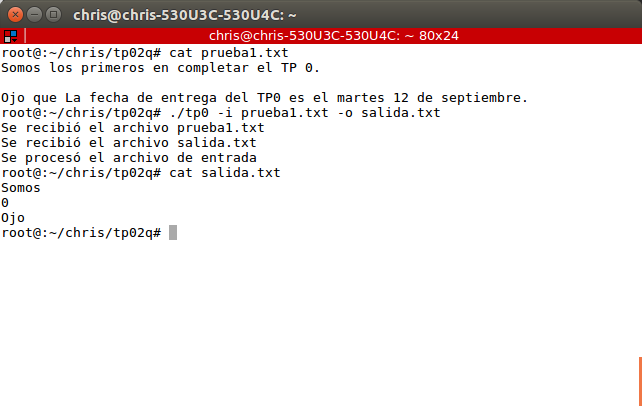
\includegraphics[width=0.5\textwidth]{prueba1.png}
\caption{Prueba utilizando archivo de entrada y salida.} \label{fig001}
\end{center}
\end{figure}

\begin{figure}[!htp]
\begin{center}
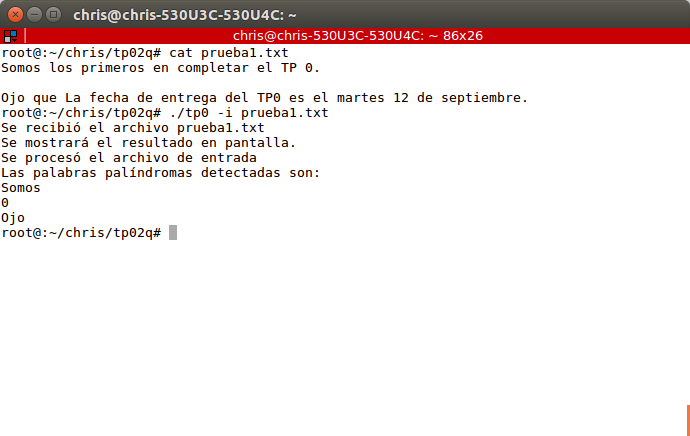
\includegraphics[width=0.5\textwidth]{prueba1SalidaPorPantalla.png}
\caption{Prueba utilizando solamente archivo de entrada.} \label{fig001}
\end{center}
\end{figure}

\begin{figure}[!htp]
\begin{center}
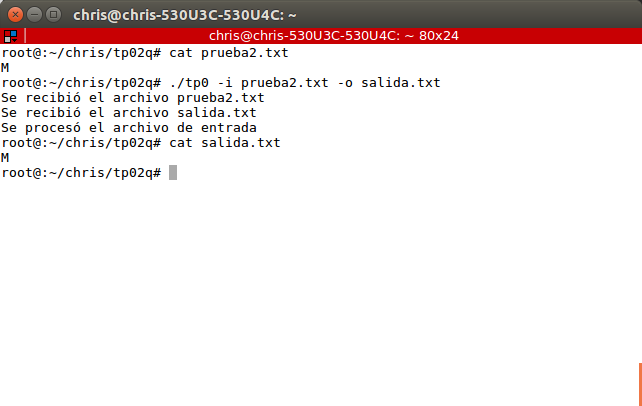
\includegraphics[width=0.5\textwidth]{prueba2.png}
\caption{Otra prueba utilizando otro archivo de entrada y salida.} \label{fig001}
\end{center}
\end{figure}

\begin{figure}[!htp]
\begin{center}
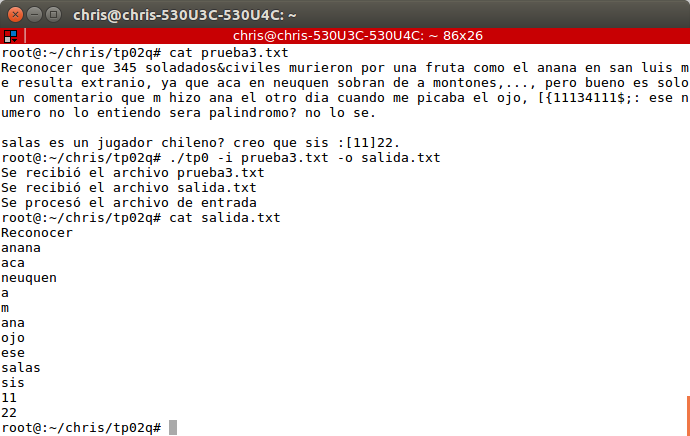
\includegraphics[width=0.5\textwidth]{prueba3.png}
\caption{Prueba utilizando otro archivo de entrada y salida.} \label{fig001}
\end{center}
\end{figure}

\begin{figure}[!htp]
\begin{center}
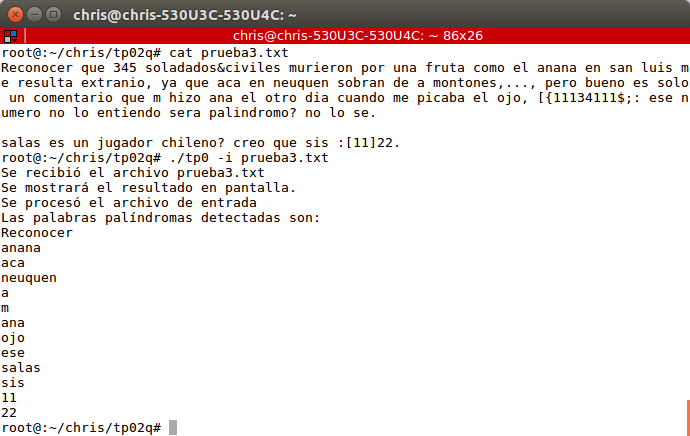
\includegraphics[width=0.5\textwidth]{prueba3salidaPorPantalla.png}
\caption{Prueba utilizando otro archivo de entrada.} \label{fig001}
\end{center}
\end{figure}

\begin{figure}[!htp]
\begin{center}
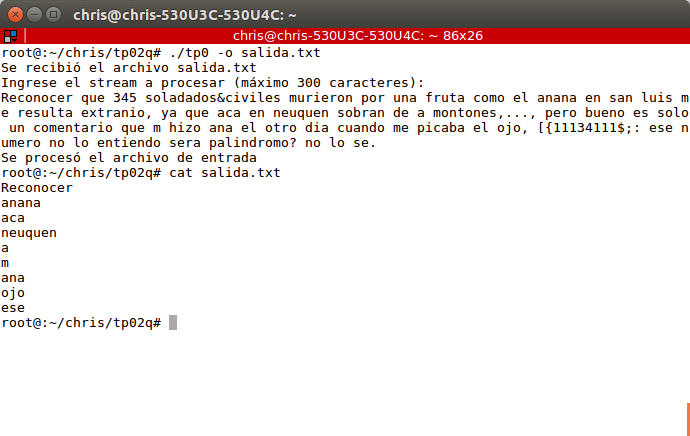
\includegraphics[width=0.5\textwidth]{pruebaPorTeclado.png}
\caption{Prueba utilizando solamente archivo de salida.} \label{fig001}
\end{center}
\end{figure}

\pagebreak
\subsection{Textos utilizados}

\paragraph{Prueba 1:}

Somos los primeros en completar el TP 0.

Ojo que La fecha de entrega del TP0 es el martes 12 de septiembre.

\paragraph{Prueba 2:}

M

\paragraph{Prueba 3:} 

Reconocer que 345 soladados&civiles murieron por una fruta como el anana en san luis me resulta extranio, ya que aca en neuquen sobran de a montones,..., pero bueno es solo un comentario que m hizo ana el otro dia cuando me picaba el ojo, [{11134111$;: ese numero no lo entiendo sera palindromo? no lo se.

salas es un jugador chileno? creo que sis :[11]22.


\section{Código MIPS generado} 

\subsection{Código fuente Assembly}
\begin{lstlisting}[language=Assembler]
    
\end{lstlisting}


\section{Conclusiones}

El trabajo práctico nos resultó interesante, no por el programa a desarrollar en sí, sino por lo que representó trabajar con el emulador GXEmul, emular la arquitectura MIPS, crear el túnel de comunicación entre el host OS (Linux, distribución Ubuntu) y el guest OS (NetBSD). Aprendimos como transferir archivos entre ambos sistemas y también ciertas cuestiones del lenguaje C con el cual no estábamos toalmente familiarizados.

\begin{thebibliography}{1}

\bibitem{lib} GetOpt library, https://www.gnu.org/software/libc/manual/html_node/Example-of-Getopt.html.

\bibitem{stack} StackOverflow, https://www.stackoverflow.com.

\end{thebibliography}

\end{document}
